\section{GECS - Graph Entity Component System}
\label{chap:3}

The following chapter introduces the GECS C Library, built with the theory introduced in chapter \ref{chap:2}. Not all code will be presented in this paper, but the implementation is freely available online [repo link]. All code presented is written by me except for the hashing function and contains zero dependencies and is C99 compatible.

\subsection{Inspiration}
Before diving into the implementation, the inspiration behind the GECS C library is obviously graphs. So it's important to understand visually how the GECS models archetypes and worlds. The ECS creates visual divisions in structures on can be parallelized and what can't. The graph GECS is modeled from is shown in Figure \ref{fig:gecs_graph}.

\begin{figure}[H]
    \centering
    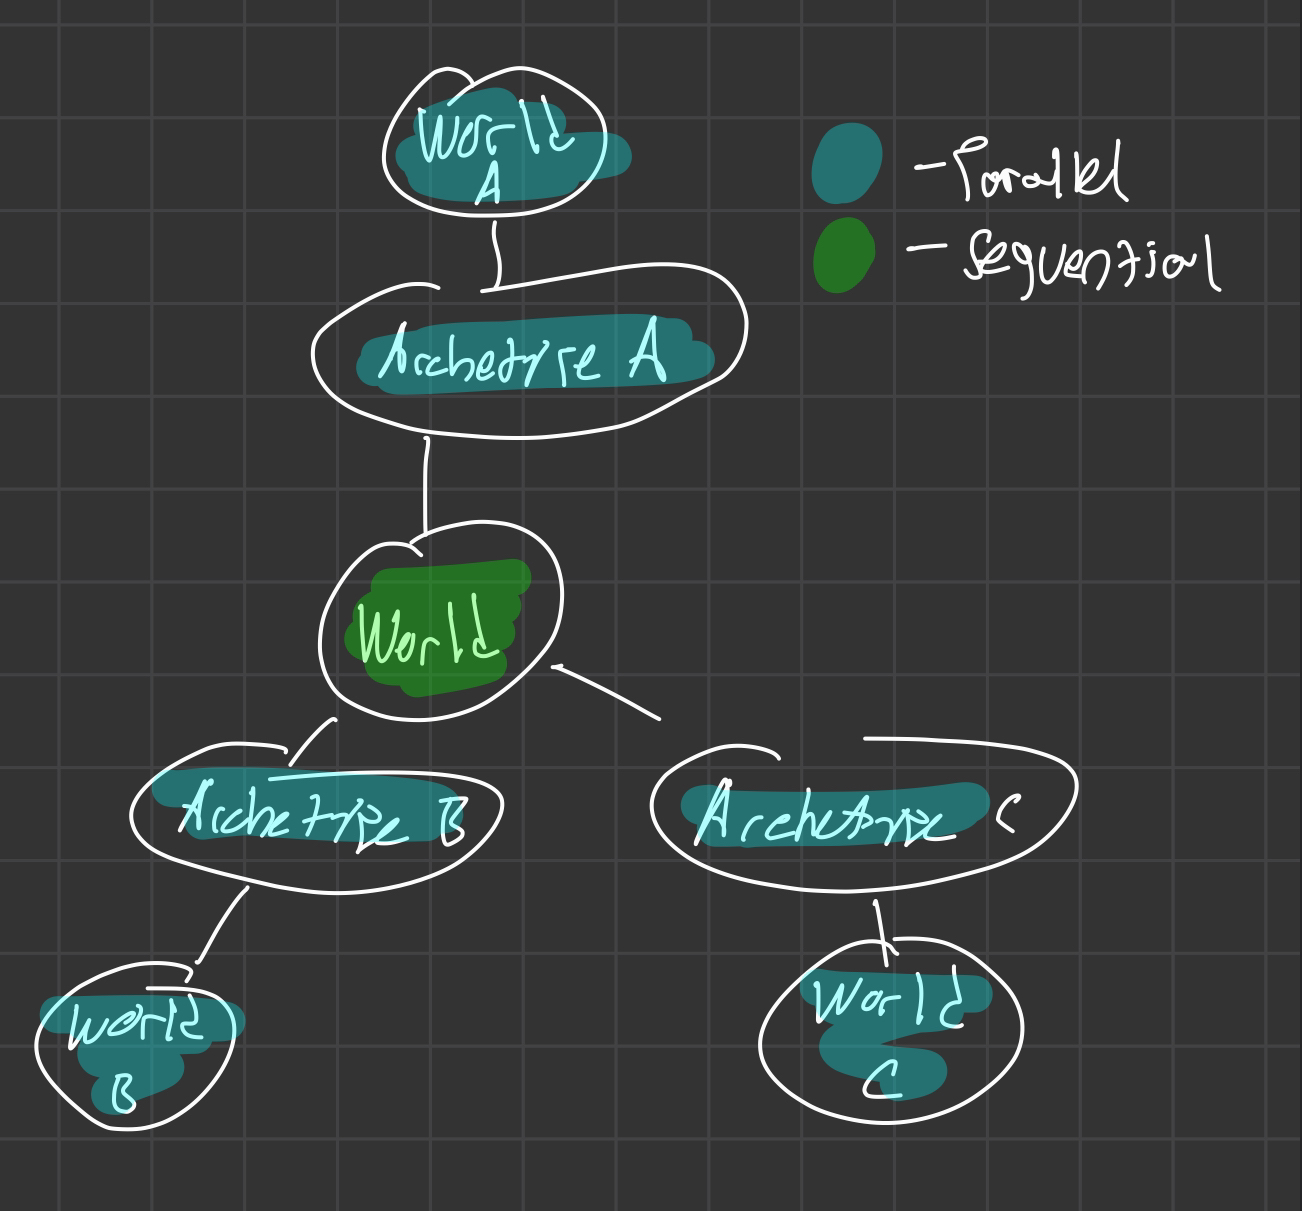
\includegraphics[width=0.5\linewidth]{resources/gecs_graph.png}
    \caption{GECS Graph Visualization}
    \label{fig:gecs_graph}
\end{figure}

In Figure \ref{fig:gecs_graph}, the graph displays the following properties:
\begin{enumerate}
    \item There is always exactly one sequential world.
    \item All archetype vertices can contain edges to other archetype vertices.
    \item All archetype vertices always contains an edge to the sequential world.
    \item All archetype vertices always contain an edge to one parallel world.
    \item A parallel world connects to one archetype, always.
    \item A parallel world cannot have an edge to another parallel world.
\end{enumerate}

The key feature of the GECS library is that each archetype simulates the events it wants to apply to the sequential world before the serialization point occurs. After the serialization point, the sequential world takes over and performs an analysis on the changes within each archtype to update itself before starting the next frame.

Effectively, the parallel worlds are the ledgers discussed in section \ref{sec:ledger} with the added benefit instead of caching operations to be done in parallel, the world simulates as if those changes are actually happening. So at the serialization point, the only operation that needs to be performed is a $\delta$ transition to another archetype for entities in the ledger.

\subsection{Data Structures}
The data structures that compose of the GECS library are vectors and hashmaps. The vector wraps contiguous elements and provides a set of functional programming style utility functions to help with code clarity. The hashmap is implemented as an open address hashing table with a load factor of $0.75$. There is nothing special about these structures and neither are thread safe. Originally, the hashmap was thread safe and was implemented using this paper \cite{hashmaps} but later found it unnecessary so it was scraped in development. 

\subsection{World Struct}
The code defined in Figure \ref{code:g_core_t} is not exactly the same code as seen on the repository on GitHub. In the actual code, the types are different in order for the C compiler to do it's magic. The types presented here are for code clarity instead of compilability.

\texttt{g\_core\_t} represents a world from the concurrency model and it's what's given to the library user to manipulate the ECS.

\subsubsection{Flags}
The \texttt{is\_main} flag checks if this world is the original or if it's a ledger. This is used through various points in the implementation as the recursive breakpoint when doing manipulations to \texttt{g\_core\_t} objects. 

The \texttt{invalidate} flag will make more sense once the archetype struct is introduced but this exists because the \texttt{map\_t} type can grow. Each archetype maintains a cache of addresses for quick access to entity data. When the map resizes, those addresses become invalid and must be recache'd. Even though this is not ideal, the map grows by a factor of 2 each time the load factor is reached, so cache invalidations do not happen often. 

The \texttt{reprocess\_fsm} flag is a flag that gets set whenever a new archetype is added to the graph. This is because the systems must get redistributed across the graph.

\subsubsection{Data}
\texttt{component\_registery} and \texttt{archetype\_registry} are maps that utilize the hashing function. This is because component ids are generated via hashing and archetypes are sets of component ids. In order to ensure the same hash is generated for sets of components in differering orders, the hashes are first sorted before the archetype is passed into a hashing function. Unfortunately there was not enough time to implement a hashset and so ordered vectors are used in their place.

\begin{figure}[H]
    \begin{lstlisting}[
        language=C
    ]
struct g_core_t {
  uint64_t id_gen;          /* Generates unique IDs */
    
  /* FLAGS */
  int8_t is_main;           /* Flag for check if parallel or sequential */
  int8_t invalidate;        /* Invalid cache before next tick */
  int8_t reprocess_fsm;     /* Flag for reprocessing the FSM before next 
                             tick. */

  /* DATA */
  map_t component_registry; /* Map: hash(name) -> comp size */
  map_t archetype_registry; /* Map: hash([name]) -> archetype */
  map_t entity_registry;    /* Map: entt id -> entt record */
    
  vec_t system_registry;    /* Vec: system_data. */
};
    \end{lstlisting}
    \caption{\texttt{g\_core\_t} struct definition}
    \label{code:g_core_t}
\end{figure}

\subsection{Archetype Struct}
The code in Figure \ref{code:archetype} represents the archetype as seen in GECS. There's many members of this so the discussion of them will be split into two groups: The implementation members and the ledger/caching members. 

\begin{figure}[H]
    \begin{lstlisting}[
        language=C
    ]
struct archetype {
  uint64_t archetype_id; /* Unique Identifier for this archetype. */
  
  vec_t type_set;   /* Ordered Vec: hash(names) */
  vec_t composite;  /* Contiguous vector of interleaved compents */
  vec_t contenders; /* Vec: system_data* */
  
  map_t offsets; /* Map: hash(name) -> interleaved comp offset */
  
  /* The following members are made for concurrency and caching purposes. */
  g_core_t *cache;               /* OOB mutations go here. */
  vec_t     entt_delete_queue;   /* Queue : entt id */
  vec_t     entt_creation_queue; /* Queue : c(entt id) */
  vec_t     dead_fragments;      /* Ordered Vec : index_of(composite) */
  
  map_t cache_interface; /* Map: entt id -> c(record) */
  map_t entt_members;    /* Map : entt id -> *record */
};
    \end{lstlisting}
    \caption{\texttt{archetype} struct definition}
    \label{code:archetype}
\end{figure}

\subsubsection{Archetype Implementation Members}
The \texttt{type\_set} member is a sorted vector containing the hashes of type ID's of the components this archetype belongs to. Hashing the bytes of this member produces the \texttt{archetype\_id}. The \texttt{composite} vector is the vector where contiguous elements of this archetype are stored. Each element is a segment of memory in which components are interleaved. The isolated member in the middle, the \texttt{offsets} table, is a table containing the offset of a particular component being queried on.  
The only member in this set related to concurrency is the \texttt{contenders} vector. This vector contains pointers to the systems that process this archetype. This cache never needs to be cleared because all systems are defined before the first tick and changes after are undefined behavior.


\begin{figure}[H]
\begin{verbatim}
Offset Table:                                                             
+-----------+-------+                                                     
|Component  |Offset |                                                     
+-----------+-------+                                                     
|Component A|     2 +------+                                              
+-----------+-------+      |                                              
|Component B|     0 +---+  |                                              
+-----------+-------+   |  |                                              
|Component C|     5 +---+--+--+                                           
+-----------+-------+   |  |  |                                           
                        |  |  |                                           
                        |  |  |                                           
Composite Vector:       v  v  v                                           
+--+--+-----+--+--+-----+--+--+-----+--+--+-----+--+--+-----+--+--+-----+ 
|  |  |     |  |  |     |  |  |     |  |  |     |  |  |     |  |  |     | 
|  |  |     |  |  |     |  |  |     |  |  |     |  |  |     |  |  |     | 
|B.|A.|C....|B.|A.|C....|B.|A.|C....|B.|A.|C....|B.|A.|C....|B.|A.|C....| 
+--+--+-----+--+--+-----+--+--+-----+--+--+-----+--+--+-----+--+--+-----+ 
|Index 0    |Index 1    |Index 2    |Index 3    |Index 4    |Index 5    | 
\end{verbatim}
\caption{Specific Component Retrieval}
\label{code:component_retrieval}
\end{figure}

\subsubsection{Archetype Caching And Ledger Members}
The rest of the members of the \texttt{archetype} struct are members related to caching and concurrency. For doing concurrent entity deletions and creations, the \texttt{entt\_deletion\_queue} and \texttt{entt\_creation\_queue} are used respectively. Other entity transitions like adding or deleting components interface with the cache. Since the cache is a seperate world, in order to access it an ID interface is required. The \texttt{cache\_interface} member maps entity ID's from the sequential world generator with that of the parallel one. The \texttt{dead\_fragments} vector contains indices of the composite vector that are no longer in use. Once entities transition out of the archetype on the merge phase, there will be indices in the vector that need the elements removed. The vector is ordered on while elements are placed in it for optimizing the defragmentation algorithm.

\begin{figure}[H]
\begin{verbatim}
+-----------+     +--------------------------------------+               
|Sequential |     | Archetype:                           |               
|World      |     |                       +-----------+  |               
|           |     | Cache Interface:      |Parallel   |  |               
|           |     | +---------+---------+ |World      |  |               
|           |     | |Entity ID|Entity ID| |           |  |               
|           |     | +---------+---------+ |           |  |               
|           |     | |Index 0  |Index 3  | | +-->      |  |               
|        ---+--+  | |         |         | | |         |  |               
|           |  |  | |Index 8  |Index 5  | | |         |  |               
|           |  +--+-+-->      |      ---+-+-+         |  |               
+-----------+     | |Index 3  |Index 4  | |           |  |               
                  | |         |         | |           |  |               
                  | +---------+---------+ +-----------+  |               
                  |                                      |               
                  +--------------------------------------+                               
\end{verbatim}
\caption{Entity Cache Interface}
\label{code:component_retrieval}
\end{figure}

\subsection{System And Entity Structs}
The following are the \texttt{system\_data} and \texttt{entity\_record} structs. The \texttt{system\_data} struct contains a function pointer \texttt{run\_system} which is provided by the user. This is the entry point into the users code. The \texttt{requirements} vector is a list of components where an archetype must have at least one to be paired. See section \ref{sec:scheduling}. The \texttt{entity\_record} contains the index at which the entities composite can be found alongside a cached pointer to the archetype this entity belongs to.

\begin{figure}[htbp]
    \begin{lstlisting}[
        language=C
    ]
struct system_data {
  g_system  run_system;     /* A function pointer to the system. */
  vec_t     requirements;   /* Vec: hash(name) */
};

struct entity_record {
  archetype *a;     /* The archetype this entity belongs to. */
  uint64_t   index; /* The index to collect their components. */
};
    \end{lstlisting}
    \caption{\texttt{entity\_record} and \texttt{system\_data} struct definition}
    \label{code:sd_and_er}
\end{figure}

\subsection{API Objects}
There are three API structs that library users interface with: The \texttt{g\_itr} struct, the \texttt{g\_query\_t} struct, and the \texttt{g\_vec} struct. 

\texttt{g\_query\_t} is passed as the single parameter to all system functions. Using this struct, a user contextually interfaces with the system currently in process. It contains three pointers: a pointer to the sequential world being processed, a pointer to the archetype, and a pointer directly to the composite for ease of use.

\texttt{g\_vec} is used by a user who confidently wants to do embarassingly parallel tasks using the libaries concurrency functions. It contains a reference to the offset table and composite.

\texttt{g\_itr} is used by a user who wants to begin querying over the components retrieved. It's a context object on how far it has progressed. Internally, it's actually just a wrapper over \texttt{g\_vec} and just adds an index counter.

\begin{figure}[htbp]
    \begin{lstlisting}[
        language=C
    ]
struct g_query_t {
  g_core_t  *world;                /* The world being queried on */
  archetype *archetype_context;    /* Which context are we running */
  vec_t     *component_store;      /* Address to composite */
};
        
struct g_itr {
  uint64_t   idx;
  g_vec     *vec;
};

struct g_vec {
  vec_t           *stored_components; /* Address to composite. */
  gid_gsize_map_t *offsets;           /* Address to table. */
};
    \end{lstlisting}
    \caption{\texttt{entity\_record} and \texttt{system\_data} struct definition}
    \label{code:apis}
\end{figure}

\subsection{API}
The GECS API is roughly inspired by how the FLECS API with how to access specific member fields. Otherwise it is of this papers own design. There are four categories of functions in the GECS API:
\begin{itemize}
    \item World Functions
    \item Thread Unsafe ECS Functions
    \item Thread Safe ECS Functions
    \item Query Functions
\end{itemize}

The header file containing the ECS defintions is linked in the Appendix \ref{appendix:a}.

\subsection{World Functions}
There are three world functions: \texttt{g\_create\_world}, \texttt{g\_progress}, \texttt{g\_destroy\_world} and each are self explanatory. \texttt{g\_progress} runs the ECS engine for exactly 1 tick.

\subsection{Thread Unsafe Functions}
The thread unsafe functions include any function that directly modifies the sequential worlds data structures. Either the maps, vectors, or \texttt{id\_gen}. There exists a thread unsafe function for all the normal entity operations: add, get, set, and remove components and create and delete entities.  

\subsection{Thread Safe Functions}

Just like how there exists a thread unsafe function for all normal entity operations, there exists a thread safe function for all normal entity operations as well. It's also important to note that all query functions are also thread safe.

\subsubsection{Query Functions}
The query functions are the set of functions used to interface and progress the runtime. The two core functions are: \texttt{gq\_vectorize} and \texttt{gq\_seq}. Depending on how the user wants their components processed, they can use the vectorize function to enable concurrent element processing on the contiguous vector or they can use the sequential function to retrieve an iterator.

\textbf{\texttt{gq\_vectorize} approach:} When using the vectorize function, the only function that can use this structure is the \texttt{gq\_each} function. This function splits the composite to be processed over multiple threads.

\textbf{\texttt{gq\_seq} approach:} After creating the \texttt{g\_itr} structure, to progress to the next element call \texttt{gq\_next} and to check if there are any elements left call \texttt{gq\_done}.

To select a component, pass in the \texttt{g\_itr} struct with the component name to \texttt{gq\_field}. 

\subsection{Examples}
In Appendix \ref{appendix:code_example_1}, there exists an example program that protrays the synchronization capabilities of GECS. It contains two systems: one which makes an entity fall to 0 and add a "Fell" component, and a system that notifies a entity fell and deletes them. Although both of these systems are dependent on eachother, they both run concurrently and produce the same results as if they were ran sequentially. The following is a print of the code:

\begin{figure}[H]
    \begin{verbatim}
Updated to 9
Updated to 9
No entity fell this tick!                            
Updated to 9
Updated to 8
No entity fell this tick!                            
Updated to 8
Updated to 8
...
...
Entity fell, deleting
Entity fell, deleting
Entity fell, deleting
\end{verbatim}
\caption{Entity Cache Interface}
\label{code:component_retrieval}
\end{figure}

Both of these systems run in parallel but the moment a transition occurs, it is cached until the serialization point. As such, all entities get deleted at the same time because all them share counters that started at the same value. The prints inbetween are proof that these systems are truely concurrent and there is no order on which systems run relative to eachother.

\subsection{Entity ID Representation}
In GECS, Entity ID's takes inspiration from the way ID's are handled in FLECS but not to the advanced extent FLECS does. One bit is reserved to understand what context an entity lives in. Because GECS needs to support entity generation inside of a system that is running concurrently, those ID's generated do not exist in the sequential world object but inside the archetype's cache. This ID is eventually scrapped for a real ID. 

In hindsight, this ID vanishing problem could easily be solved by using an atomic integer generator instead of entirely simulating the worlds. 


\begin{figure}[H]
\begin{verbatim}
                64                                     0                                
                +------------------------------------+-+                                
                |Entity                              | |                                
                |ID Bits                             | |                                
                +------------------------------------+-+                                
                 Context                               ^                                
                 Bit  ---------------------------------+                                
                        0 = Sequential Context                                        
                        1 = Parallel Context                                          
\end{verbatim}
\caption{Entity Cache Interface}
\label{code:component_retrieval}
\end{figure}

An associated set of macros are defined in \texttt{gid.h} that contain macros for bit manipulation over entity ID's.

\subsection{The Tick Lifecycle}
The tick lifecycle is processing exactly one tick, or one time, the \texttt{g\_progress} function. The cycle is split into three parts: the preparation, execution, and cleanup phases. Both the preparation and cleanup phases are done sequentially on the main thread, while the execution phase is where threads are scheduled to run systems.

The preparation phase only has one job which is to ensure the validity of the entity FSM before systems start modifying it. This is done by checking the \texttt{reprocess\_fsm} flag.

The execution phase starts by collecting all archetypes and iterating over them to reach their \texttt{contenders} vector. This vector contains pointers to the \texttt{system\_data} structs. Once loaded, threads will by scheduled to run the system process.

The cleanup phase is where the majority of the work occurs for GECS. It must do 4 things:
\begin{itemize}
    \item Check if cache requires invalidation
    \item Migrate temporary entities out of the caches
    \item Clear the caches to prepare for the next tick
    \item Defragment all composites that have unreference-able indices.
\end{itemize}

The cleanup phase algorithms for defragmentation and cache clearance are written into this section. The following sections will contain the algorithms for entity migration, Entity FSM processing, and scheduling refrenced here.

\subsubsection{Defragmentation}
Defragmentation is the process of re-vectorizing a composite such that all elements in the vector are referenced by one entitiy. In order to achieve this: the entities who have either been deleted or transitioned away from this archetype must have their composite index loaded and then removed from the vector. Because vector deletion is $O(N)$ time, if $e$ amount of entities are deleted, then the defragmentation algorithm will take $O(N^e)$ which is not feasible. 

As such, the vector \texttt{dead\_fragments} is used. When an entity leaves this archetype, the index to delete is pushed into \texttt{dead\_fragments}. The following algorithm can be used to defragment the vector in $O(N)$ time for $e$ indices.

\begin{figure}[htbp]
    \begin{enumerate}
        \item Create vector \texttt{out}
        \item Create vector \texttt{rolling\_offsets} and integer \texttt{dead\_index}.
        \item For each element $ e \in \texttt{composite}$, do the following
        \item If the index of $e$ is dead, do the following steps 5-7:
        \item Increment \texttt{dead\_index}
        \item Push $\texttt{rolling\_offsets} \leftarrow \texttt{dead\_index}$
        \item Continue
        \item Push $\texttt{rolling\_offsets} \leftarrow \texttt{dead\_index}$
        \item Push $\texttt{out} \leftarrow e$
    \end{enumerate}
    \caption{Defragment Algorithm Part 1}
    \label{alg:defrag1}
\end{figure}

In the algorithm in Figure \ref{alg:defrag1}, it produces two new vectors: the \texttt{out} and \texttt{rolling\_offsets} vector. The \texttt{out} vector is the newly defragmented vector that will replace the old one. The \texttt{rolling\_offsets} vector represents a translation map between the old vector indices and the new vectors indices. Since the elements of the \texttt{composite} and \texttt{out} have elements sorted in the same order, the \texttt{rolling\_offsets} counts the difference between those two vectors.
                  
\begin{figure}[H]
\begin{verbatim}
    Original                                        Dead                     
    Vector                                          Fragments                
    +-----+-----+-----+-----+-----+-----+-----+     +-----+                  
    |  A  |  B  |  C  |  D  |  E  |  F  |  G  | +---+  2  |                  
    +-----+-----+-----+-----+-----+-----+-----+ |   +-----+                  
    0     1     2     3     4     5     6       | +-+  3  |                  
                +-------------------------------+ | +-----+                  
                |                                 | |  5  |                  
    Offset      |     +---------------------------+ +--+--+                  
    Vector      v     v                                |                     
    +-----+-----+-----+-----+-----+-----+-----+        |                     
    |  0  |  0  |  2  |  2  |  2  |  3  |  3  |        |                     
    +-----+-----+-----+-----+-----+-----+-----+        |                     
    0     1     2     3     4     5     6              |                     
                                  ^                    |                     
                                  +--------------------+   
\end{verbatim}
\caption{Offset Vector Diagram}
\label{code:component_retrieval}
\end{figure}

With this offset vector, all entity records found in the archetype \texttt{entt\_members} are then loaded and then a subtraction operation is performed between the index and the offset value at that index as well. 

\begin{figure}[H]
\begin{verbatim}
    Offset                                                                  
    Vector                                                                  
   0+-----+     Entity Record                      Entity Record            
    |  0  |     Table                              Table                    
   1+-----+     +-----+-----+                      +-----+-----+            
    |  0  |     |ID   |Index|                      |ID   |Index|            
   2+-----+     +-----+-----+ index - offset(index)+-----+-----+            
    |  2  |     |0    |1    +--------------------->|0    |  1  |            
   3+-----+     +-----+-----+ index - offset(index)+-----+-----+            
    |  5  |     |1    |4    +--------------------->|1    |  2  |            
   4+-----+     +-----+-----+ index - offset(index)+-----+-----+            
    |  3  |     |2    |6    +--------------------->|2    |  3  |            
   5+-----+     +-----+-----+                      +-----+-----+            
    |  3  |     |. . .|. . .|                      |. . .|. . .|            
    +-----+     +-----+-----+                      +-----+-----+            
 Original             |                      Defragment  |                  
 Vector+--------------+--------------+       Vector+-----+-----+            
       v                 v           v             v     v     v            
 +-----+-----+-----+-----+-----+-----+-----+ +-----+-----+-----+-----+      
 |  A  |  B  |  C  |  D  |  E  |  F  |  G  | |  A  |  B  |  E  |  G  |      
 +-----+-----+-----+-----+-----+-----+-----+ +-----+-----+-----+-----+      
 0     1     2     3     4     5     6       0     1     2     3            
\end{verbatim}
\caption{Update Entity Record With Offset Mapping Diagram}
\label{code:component_retrieval}
\end{figure}

This was part two of the defragmentation algorithm. At the end of this procedure, the composite vector is completely vectorized and ready for the next tick.

\subsubsection{Cache Clearance Algorithm}
Cache clearance is fairly straightforward since all that needs to be done is apply the \texttt{clear} function to both vectors and maps. Given that the starting point is the sequential world object, the following are cleared by the clear cache function:

For archetypes:
\begin{itemize}
    \item entt\_delete\_queue
    \item entt\_creation\_queue
    \item cache\_interface
\end{itemize}

For archetype caches:
\begin{itemize}
    \item entity\_registry
    \item archetype\_registry
\end{itemize}

For archetypes caches archetypes:
\begin{itemize}
    \item composite
    \item entt\_members
\end{itemize}

Remember that archetype caches are of the same struct as the sequential world and is a world object itself. The last set of clears only occurs inside the parallel worlds.

\subsection{Entity FSM}

\subsubsection{Concurrent Entity Component Additions}
\subsubsection{Concurrent Entity Component Deletions}
\subsubsection{Entity Consolidation Algorithm}

\subsection{Caches}

